\chapter{LPWAN e Lora}
Nel seguente capitolo si approfondirà il concetto di rete \emph{LPWAN} e la sua
struttura, andando ad analizzare i vari layer di cui è composta. 
In particolare si farà riferimento alla tecnologia Lora che implementa questo
tipo di rete, andandone ad analizzare i vari componenti, quali
\begin{itemize}
\item layer fisico
\item la composizione dei pachetti 
\item le classi di devices implementati
\end{itemize}

\section{LPWAN}
Tra le varie tipologie di rete emergenti per l'IoT, LPWAN sta riscuotendo sempre
più interesse. Questo tipo di rete si basa sulla topologia a stella, la quale
permette di avere un elevato numero di devices connessi ad una sola stazione
base.Inoltre per la sua struttura LPWAN supporta comunicazioni a lungo raggio
risultando adatta per i vari \emph{use-case} del internet of things. I due
principali concorrenti che implementano queste tecnologie sono Sigfox\tm e
Semtech\tm possessore di Lora\tm. L'implementazione proposta da Sigfox utilizza
la Ultra Narrow Band tramite la quale è possibili inviare messaggi con payload
lungo 12 \emph{byte} in 6 secondi usando una frequenza di 100[Hz]. Per via delle
varie regolazioni, utilizzando la tecnologia Sigfox si ha un numero limitato di
messaggi per giorno.
Al contrario la tecnologia Lora, implementa \emph{spread spectrum Physical
Layer} (PHY) il quale permette una maggiore ricezione andando ad influire sul
data-rate possibile

\section{Lora}
\emph{Lora} è una tecnologia semi-proprietaria, sviluppata da Semtech. Lora è
composta da un parte proprietaria detta \emph{Lora}\cite{LoRaCss101} la quale definisce il layer
fisico, e una parte libera chiamata LoRaWAN\cite{LoRaWAN101}.
\improvement[inline]{Completare e riscrivere}


\section{CSS}
Alla base del layer fisico troviamo la modulazione (CSS), questo tipo di
modulazione della frequenza, utilizzata anche in altre applicazioni radio, 
esempio radar ecc..\improvement{Aggiungere qualche altro esempio}.
Questo tipo di modulazione ha numerosi vantaggi quali 
\begin{itemize}
\item Uno spettro idealmente rettangolare, il quale utilizza tutta la capacità
del canale e fornisce un ottima densità spettrale di potenza rispetto agli atri
tipi di trasmissione.
\item \textbf{Segnali di tipo Chirp} possono essere sovrapposti in modo tale da
poter variare il data-rate e l'energia per bit in modo adattativo per aumentare
l'efficienza complessiva.
\item \textbf{Hanno guadagno programmabile}, il quale permette di raggiungere
distanze considerevoli mantenendo un buon SNR .
\item  \textbf{Ottima risoluzione nel asse del tempo}, quindi ottimi per coprire
lunghe distanze.
\item \textbf{Immuni al effetto Doppler} 
\item \textbf{Immuni al degenerazioni per effetto di multipath} \info{Trovare
termine per multipath}
\end{itemize}
Un segnale di tipo \emph{Chirp} assume valori compresi nella banda di frequenza
$B = [f_0,f_1]$, il suo andamento è di tipo monotono , crescente o decresente
compreso tra le due frequenze $f_0$ e $f_1$.

\begin{figure}[h]
\centering 
\input{Images/Chirp.pdf_tex}
\caption{Segnale Chirp nel dominio della frequenza}
\end{figure}
\begin{figure}[h]
\centering 
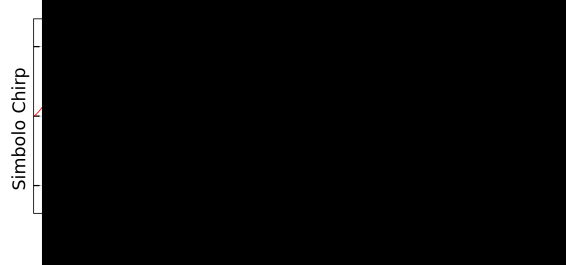
\includegraphics[width=10cm]{Time_Chirp}
\caption{Simbolo codificato col metodo Chirp nel dominio del tempo}
\end{figure}

Il numero di bit codificati in un simbolo è come detto prima un parametro
modificabile in base alle varie esigenze.


Modulazione \emph{Chirp Spread Spectrum} (CSS). La banda di frequenze utilizzate
è quella ISM. La specifica LoRa definisce LoRaWAN\cite{LoRaWAN101}, la quale
descrive il protocollo (MAC) proprietario. Il MAC layer definisce tre classi di
devices, ognuno dei quali ha un diverso use-case.

